% !TeX root=main.tex
\chapter{نتیجه‌گیری و پیشنهادات}
\thispagestyle{empty}

\section{نتیجه‌گیری}

با توجه به نتایج به دست‌آمده از آزمایش‌های انجام شده مشاهده می‌شود 50 درصد اتصالات کم‌وزن شبکه
\lr{LXMERT}
تاثیر چندانی بر کارایی نهایی شبکه ندارند. بنابراین برای کاهش پارامتر‌ها و اندازه شبکه حذف اتصالات کم‌وزن یکی از بهترین روش‌های ممکن است. ولی اگر اتصالات به صورت تصادفی اتخاب شود نتایج متفاوت است. بدین معنی که علاوه بر اتصات نوع اتصالاتی که در زیرشبکه هرس شبکه نگه می‌داریم عاملی مهم و تاثیر گذار است. در شکل \ref{ex_result} خلاصه نتایج سه نوع هرس معرفی شده به تفکیک میزان هرس و بر اساس نوع هرس قابل مشاهده است. همچنین در جدول \ref{res_all} اعداد دقیق برای بررسی‌های احتمالی گزارش شده است.

\begin{table}[ht]
	\caption{نتایج مدل هرس‌شده آموزش دیده برای انواع هرس به تفکیک درصد حذف اتصالات}
	\label{res_all}
	\centering
	\onehalfspacing
	\begin{tabular}{|c|c|c|c|}
		\hline درصد هرس & اتصالات با وزن کم & رندوم & اتصالات با وزن زیاد\\ 
		\hline 10 & $69.94 \pm 0.03$ & $69.58 \pm 0.02$  &  $69.75 \pm 0.13$\\ 
		\hline 20 & $69.59 \pm 0.11$ & $62.21 \pm 0.06$  &  $69.17 \pm 0.09$\\ 
		\hline 30 & $69.23 \pm 0.07$ & $60.23 \pm 0.24$  &  $68.60 \pm 0.08$\\ 
		\hline 40 & $68.70 \pm 0.05$ & $57.49 \pm 0.62$  &  $67.87 \pm 0.18$\\ 
		\hline 50 & $67.44 \pm 0.14$ & $52.63 \pm 0.13$  &  $67.78 \pm 0.04$\\ 
		\hline 60 & $63.94 \pm 0.01$ & $48.68 \pm 0.00$  &  $58.76 \pm 0.63$\\ 
		\hline 70 & $58.50 \pm 0.04$ & $44.96 \pm 0.34$  &  $52.28 \pm 0.26$\\ 
		\hline 80 & $50.63 \pm 0.21$ & $24.36 \pm 0.26$  &  $46.54 \pm 0.15$\\ 
		\hline 90 & $28.12 \pm 4.02$ & $24.36 \pm 0.26$  &  $25.40 \pm 0.77$\\ 
		\hline 
	\end{tabular} 
\end{table}

\begin{figure}[H]
	\center{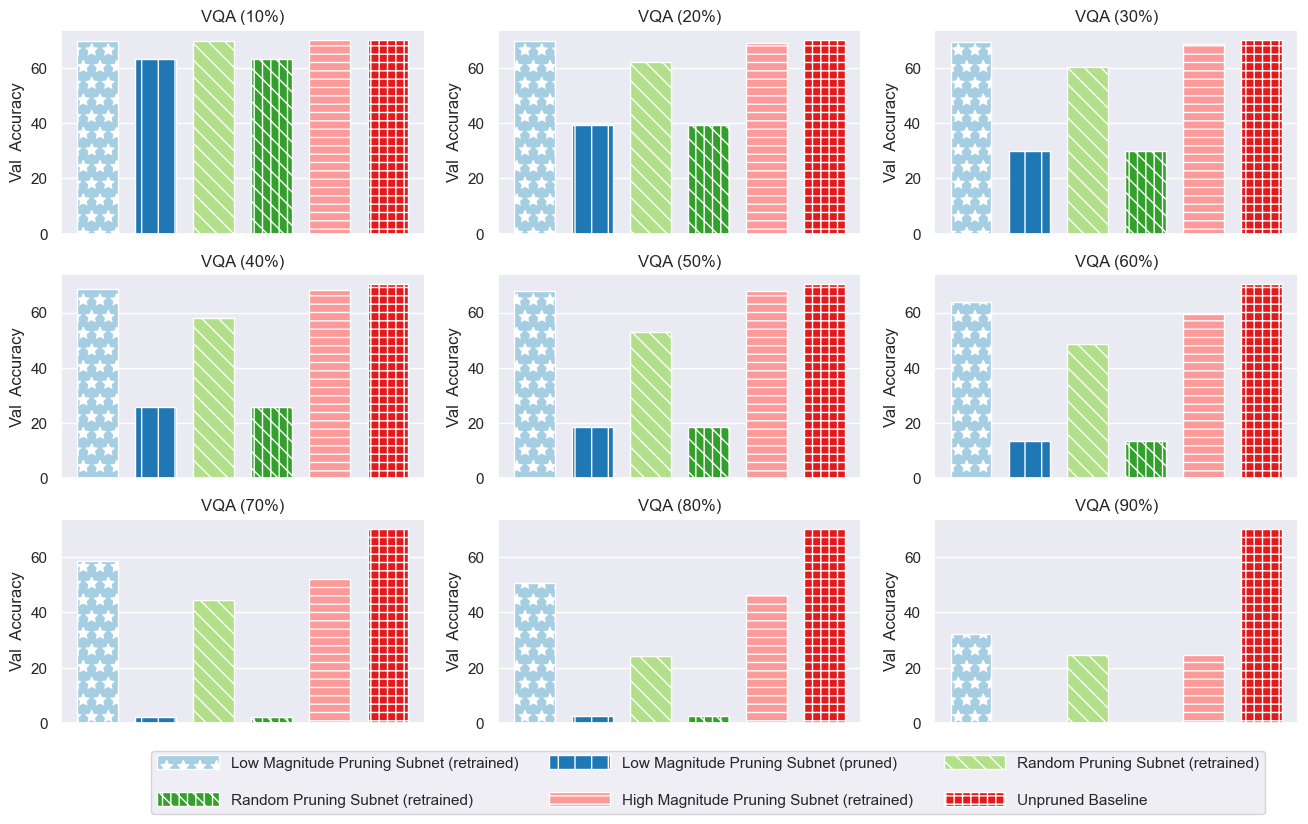
\includegraphics[width=1\linewidth]{images/experiment_result.PNG}}
	\caption{نتایج انواع هرس به تفکیک درصد حذف اتصالات}
	\label{ex_result}
\end{figure}

\section{پیشنهادات و کار‌های آینده}
با توجه به پیشرفت چشم‌گیر در هوش مصنوعی و حرکت سریع به سمت استفاده از ابزار‌های هوشمند، برای ادامه تحقیقات موارد زیر پیشنهاد می‌شود.
\begin{enumerate}
	\item در این پژوهش مدل
	\lr{LXMERT}
	بر روی مجموعه داده
	\lr{VQA}
	بررسی شد. در ادامه می‌توان دو مجموعه داده دیگر از جمله
	\lr{GQA}
	و 
	\lr{NLVR2}
	را بررسی کرد.
	\item
	می‌توان کارایی شبکه هرس شده و آموزش دیده روی مسئله 
	\lr{VQA}
	را بر روی سایر مجموعه داده‌ها
	\lr{(GQA, NLVR2)}
	 بررسی نمود. بدین ترتیب تاثیر انتقال یادگیری
	\LTRfootnote{\lr{Transfer Learning}}
	 در 
	\lr{LXMERT}
	مشخص می‌شود.
	\item روش بررسی شده در این پژوهش، هرس اتصالات شبکه می‌باشد. از این رو زمان اجرا ابتدا به انتها شبکه تفاوتی چندانی نمی‌کند. می‌توان انواع دیگر هرس از جمله هرس ساختاری
	\LTRfootnote{\lr{Structural Pruning}}
	را مورد بررسی قرار داد.
%		\lr{head attention}
	\item
	نتایج به دست‌آمده در روش اتصالات با وزن زیاد (بخش \ref{high_mag_pruning}) دور از انتظار بود. می‌توان در ادامه تحقیقات معماری شبکه
	\lr{LXMERT}
	را به صورت دقیق‌تر بررسی کرد. این بررسی ممکن است به معرفی مدل دیگری با ساختار جدید و بهبود دقت در مسئله پرسش و پاسخ تصویری ختم شود.
	\item بیشتر پژوهش‌ها در موضوع فشرده‌سازی شبکه به صورت تئوری است. وقت آن است  نتیجه این پژوهش‌ها در عمل و برنامه‌های کاربردی
	\LTRfootnote{\lr{Application}}
	 مورد استفاده در روزمره انسان‌ها مورد بررسی قرار گیرد. 
	
	\item مجموعه داده
	\lr{VQA}
	که در آزمایش‌ها مورد استفاده قرار گرفت به زبان انگلیسی می‌باشد. با توجه به نبود مجموعه داده مناسب به زبان فارسی، یکی دیگر از کار‌های ارزشمند جمع‌آوری مجموعه داده فارسی پرسش و پاسخ تصویری می‌باشد. بدین ترتیب برنامه‌های کاربردی طراحی شده برای کمک به کم‌بینایان، نابینایان یا استفاده‌های دیگر می‌توانند به زبان فارسی باشند.
\end{enumerate}



